\subsection{Mechanical Readouts and Replica-Level Summaries}
Mechanical trajectories are characterized directly from saved coordinates, cohesive-link counts, and filopodial attachments. Let $\mathcal H_s(t_m)$ be the planar convex hull of all fibrin-node and platelet-center positions in slab $s$, and let $a_s(t_m)=|\mathcal H_s(t_m)|$. The clot-level envelope contraction is
\begin{equation}
C_{A,\mathrm{env}}(t_m)
=1-\frac{\sum_{s=1}^{m}a_s(t_m)}{\sum_{s=1}^{m}a_s(0)}.
\label{eq:mechanics-envelope}
\end{equation}
This is the normalized loss of the center-position envelope, without padding or rasterization. It is not solid area, porosity, or an intersection of slab interiors. The normalization weights slabs by their initial envelope area; negative values, if present, represent expansion and are not truncated.

For $N_{n,s}$ fibrin nodes and $E_{\mathrm{coh},s}(t_m)$ active cohesive links, the mean cohesive degree is
\begin{equation}
\overline{k}_{\mathrm{coh}}(t_m)
=\frac{2\sum_{s=1}^{m}E_{\mathrm{coh},s}(t_m)}{\sum_{s=1}^{m}N_{n,s}}.
\label{eq:mechanics-cohesive-degree}
\end{equation}
Each undirected link contributes one incidence to each endpoint. Original backbone edges are excluded from this degree. The active count saved at each frame is used, rather than the final cumulative link list, so links created later do not contribute to earlier states.

The attached-arm fraction is
\begin{equation}
q_{\mathrm{att}}(t_m)
=\frac{\sum_s N_{\mathrm{att},s}(t_m)}{\sum_s N_{\mathrm{arm},s}},
\label{eq:mechanics-attachment}
\end{equation}
where $N_{\mathrm{arm},s}$ sums the actual fixed arm counts of the platelets in slab $s$ and $N_{\mathrm{att},s}$ counts their valid attached-node indices. Unused padded storage slots are excluded. This observable measures attachment occupancy, not traction magnitude or the persistence of a particular attachment.

Every clot-level observation combines all $m$ slabs at the same saved time. Across replicas, clots receive equal weight, and summaries report the arithmetic mean and sample standard deviation. Slabs and successive frames are not treated as independent replicas. Comparisons at $m=8$ use the same seed blocks across force settings; comparisons across slab counts use distinct seed blocks. All comparisons are descriptive.

\subsection{Virtual Sections of Three Volumetric Clots}
For comparison with the six $m=8$ clots at $f_0=2.233$~nN, we analyzed three independently simulated cylinders adapted from the model of Michael et al.~\cite{Michael2023,MichaelCodeOcean2023}. We divided each cylinder's $32~\mu\mathrm m$ axial extent into eight $4~\mu\mathrm m$ sections. In the primary comparison, each fibrin node and platelet center was assigned to its section in the first saved frame (0.01~s) and tracked by identity through 30~min. We projected the centers onto the $xy$ plane and calculated Eq.~\eqref{eq:mechanics-envelope} relative to that first frame. We also held the section boundaries fixed and reassigned centers by their current depth at each time. These are two measurements on each clot; the replicate is the cylinder.

To check whether contraction extended beyond the hull boundary, we measured the mean squared in-plane distance of fibrin nodes from their own slab centroid. We averaged these values equally over the eight slabs, took the square root, and reported the fractional decrease of this radius relative to the first frame. The three-dimensional comparison retained initial section membership.

For the morphology comparison we used fixed sections, corresponding to repeated images at the same depth (Fig.~\ref{fig:virtual-sectioning-method}). We clipped each original fibrin backbone segment to the section before projecting it onto the $xy$ plane. A platelet contributed a profile if its spherical body intersected the section; we projected only the part inside the section. A platelet could therefore appear in two neighboring sections. In the planar model we used the original backbone and the full platelet disks. For each clot we divided the projected backbone length lying inside the union of platelet profiles by the total projected backbone length, summing both lengths over the eight slabs. Cohesive links were excluded. This measures overlap in projection: objects at different depths can overlap in the image without touching.

\begin{figure*}[!tp]
\centering
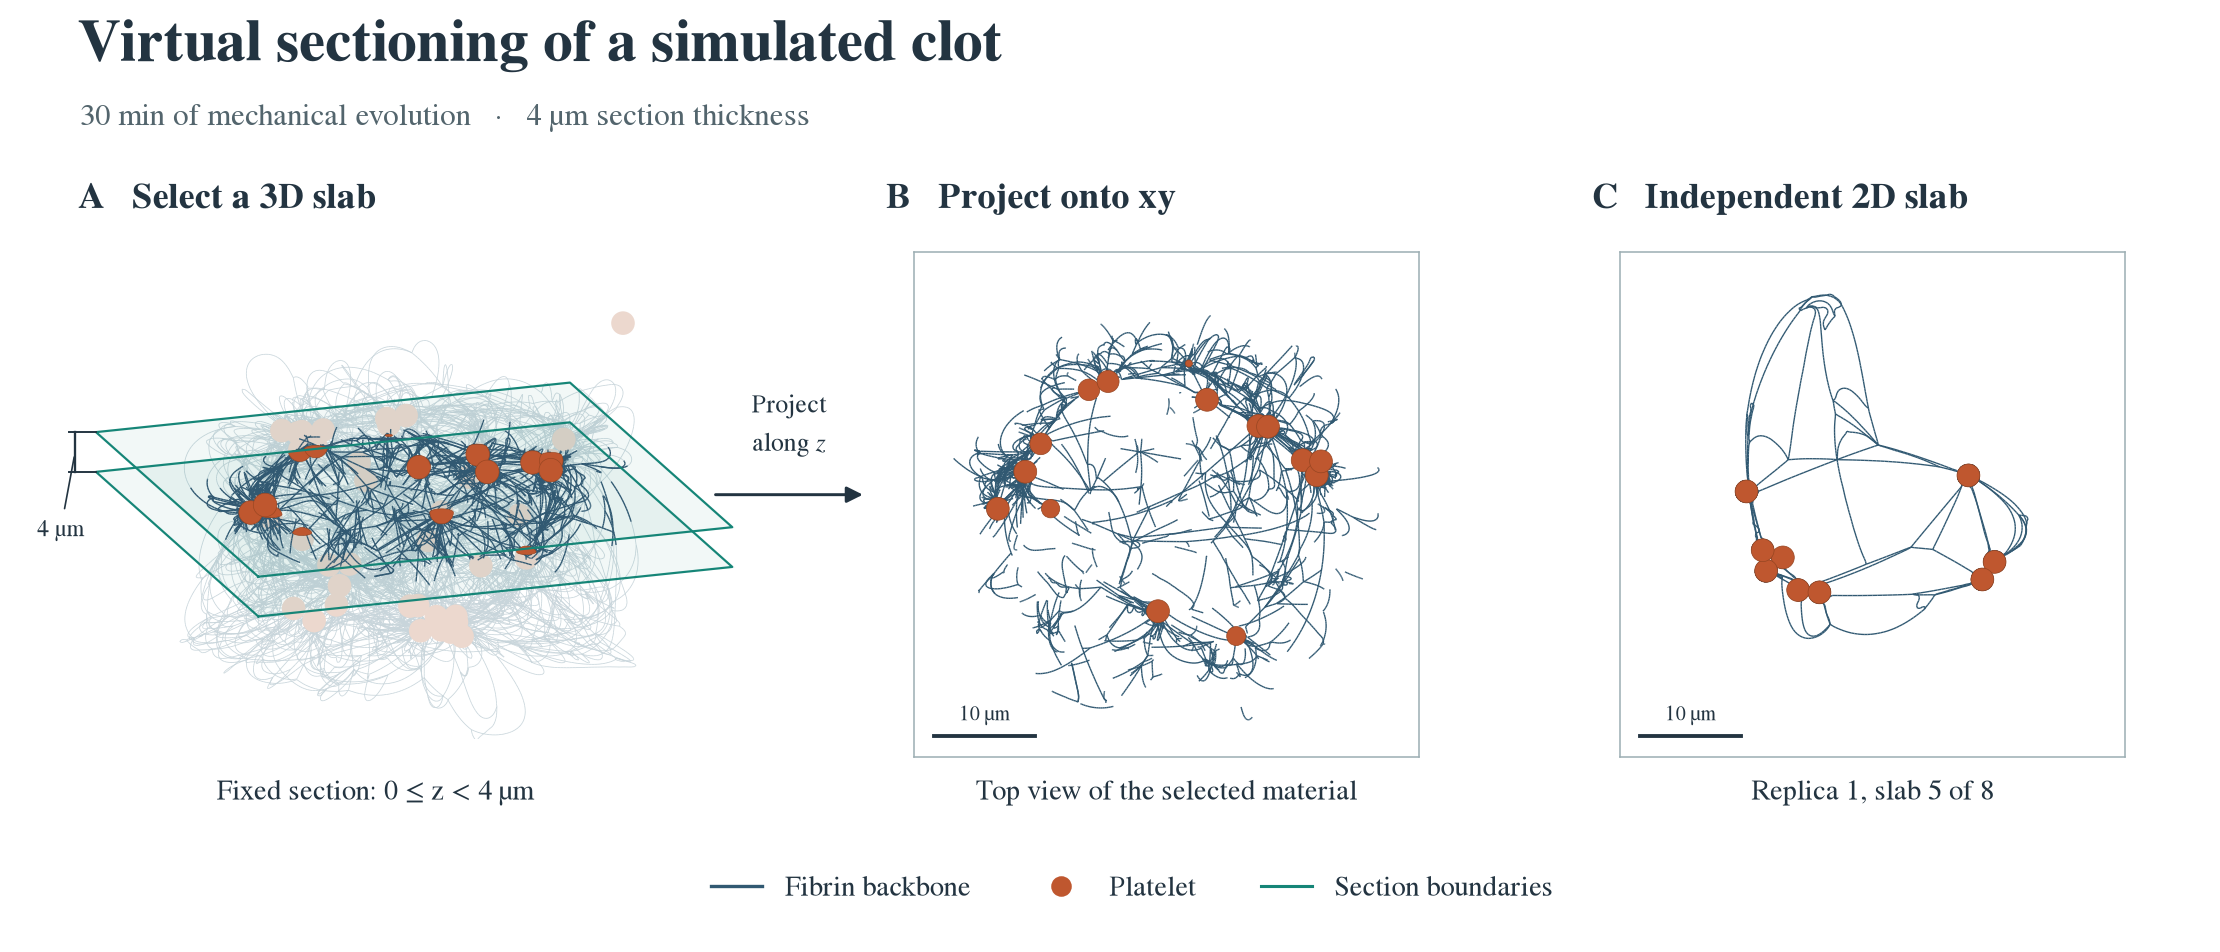
\includegraphics[width=\textwidth,trim=0bp 0bp 0bp 61bp,clip]{figures/virtual_microscopy_30min.png}
\caption{Virtual sectioning at 30~min of mechanical evolution. (A) The two planes bound a $4~\mu\mathrm m$ section of the simulated 3D clot. (B) The material inside that section is viewed along $z$: its $x$ and $y$ coordinates are unchanged. This is a projection, not a mechanical compression. (C) An independently simulated planar slab ($m=8$, $f_0=2.233$~nN) is shown at the same time and scale as (B).}
\label{fig:virtual-sectioning-method}
\end{figure*}
